\documentclass[11pt,a4paper]{article}
\usepackage[margin=25mm]{geometry}
\usepackage{graphicx,booktabs,tabularx}
\usepackage[hidelinks]{hyperref}
\title{ReVive: Explainable Financial Anomaly Detection\\\large UCS503P Prototype Stage Progress Report}
\author{Aakriti Sharma (1024030430) \and Koena (1024030831) \and Mayur Goyal (1024030828)}
\date{Thapar Institute of Engineering and Technology}
\begin{document}
\maketitle
\begin{abstract}
The ReVive prototype established the path from a transaction file to a ranked alert with a feature-level explanation and saved history. This report records the scope demonstrated at the prototype stage, the design artifacts, exploratory evidence, and the decisions carried into the final iteration.
\end{abstract}

\section{Problem and stage objectives}
ReVive was proposed for reviewers who need both a ranked set of suspicious windows and a way to inspect why an alert scored highly. The prototype focused on making that workflow observable. It aimed to run a repair detector on transaction windows, show a classical benchmark for context, and connect the score to a triage tier, feature errors, and alert storage. The final volume of alerts, repeatable evaluation, and deployment were later-stage goals.

\section{Development milestones and responsibilities}
\noindent\begin{tabularx}{\linewidth}{@{}lX@{}}
\toprule
Workstream & Prototype evidence and progress\\
\midrule
Detection engine & Koena reviewed JuRe, implemented the repair architecture, checked its structure against the paper, trained on financial inputs, and documented debugging in the weekly journal.\\
Methodology & Aakriti explored classical detectors and ensemble score normalization, examined the benchmark comparison, and documented interpretation and limitations.\\
Delivery & Mayur organized the repository and design diagrams, built the initial Streamlit workflow, debugged label recognition and table rendering, and assembled presentation materials.\\
\bottomrule
\end{tabularx}

The initial system was demonstrated through the prototype deck and application views. The submitted deck's roadmap retained a corrected baseline, explainability evaluation, integration, and broader evaluation as future work. These items describe the prototype plan. The final report records the scope ultimately delivered.

\section{System design and implementation}
\subsection{Pipeline and code structure}
The dashboard accepts synthetic input or a CSV and provides a training and scoring action. Preprocessing identifies label and numeric feature columns and creates sliding windows. A compact learned repair model reconstructs input windows. The scoring stage compares the reconstruction with the observed window using complementary discrepancies. The dashboard presents a timeline and highlights windows that cross review thresholds.

The prototype separates responsibilities into data preparation, the repair model and training loop, structural scoring, baseline evaluation, feature explanations, triage, and the Streamlit application. Classical detectors provide a comparison on the evaluated samples. SQLite records alerts so the reviewer can revisit the recent scoring history. Feature contribution and peak timestep provide a bridge from an aggregate score to the particular window needing review.

\subsection{Design artifacts}
The \href{https://github.com/aakritisharma001/ucs503p-202627-ReVive/blob/master/project-report-prototype-stage/ReVive-prototype.pdf}{prototype presentation} provides the design figures and prototype evidence. The following mapping identifies what each artifact clarifies.

\noindent\begin{tabularx}{\linewidth}{@{}lX@{}}
\toprule
Figure & Question addressed\\
\midrule
Use case (page 6) & How a reviewer starts scoring and inspects the flagged results.\\
Activity (page 7) & Where validation, scoring, triage decisions, and explanations occur.\\
Class (page 8) & How the deployed repair model, residual block, and training dataset relate.\\
Level 0 and Level 1 data flow (page 9) & How transaction input becomes scores, explanation output, and persisted alert metadata.\\
Sequence (page 10) & The order of interactions in a successful Streamlit scoring run, from Python scoring to SQLite alert storage.\\
\bottomrule
\end{tabularx}

\begin{figure}[htbp]
\centering
\includegraphics[page=7,width=0.92\linewidth]{ReVive-prototype.pdf}
\caption{Prototype activity diagram from the team's presentation. It follows the decision from scoring to explanation and alert storage.}
\end{figure}

\section{Prototype demonstration and evaluation}
The original presentation shows the alert view and an exploratory comparison with Isolation Forest and LOF. These preliminary figures depended on the selected slice and preprocessing. The prototype was evidence that the full interaction was feasible. The final report supplies the repeatable comparison with a documented chronological split and calibration policy.

\noindent\begin{tabularx}{\linewidth}{@{}lXX@{}}
\toprule
Objective & Evidence available & Outcome at this stage\\
\midrule
Run a batch end to end & Data preview, training action, and scored results & Core workflow demonstrated.\\
Show a comparative result & Preliminary chart in the prototype presentation & Comparison available for exploration. Split and leakage controls required revision.\\
Explain a flag & Feature contribution and peak-timestep example & A numeric explanation could be inspected. Domain semantics remained limited.\\
Save alerts & SQLite workflow and history display in prototype materials & Local storage integrated. Fresh-session evidence belongs to final verification.\\
\bottomrule
\end{tabularx}

\section{Challenges, mitigation, and next iteration}
Labels must be detected consistently and excluded from inputs. The final build will validate binary labels, split chronologically before fitting preprocessing, and exclude anomalous windows from normal training while keeping original row adjacency. This will reduce the risk of a benchmark that benefits from information from the evaluation partition.

The team explored an ensemble baseline and identified the problems with averaging scores on different scales. The final evaluation will report the individual classical baselines and document which comparison configuration was actually used. For the review workflow, fixed cutoffs will be compared with percentiles from normal validation scores. The verification record will capture alert counts, precision, recall, seed, split, settings, and persistence.

The dashboard may stall on large data or dense windowing. Bounded examples and batched scoring will keep the lab walkthrough practical. Anonymized features and unusual legitimate behavior will continue to limit how alerts can be interpreted. The scope of the next release is a batch review tool suitable for a course demonstration.

\section{Conclusion}
The prototype delivered a working review path and exposed weaknesses in evaluation and deployment that could be addressed independently of the core model. The final iteration prioritizes methodological correctness, repeatable evidence, and an accessible demonstration.

\appendix
\clearpage
\section{Class diagram}
\begin{center}
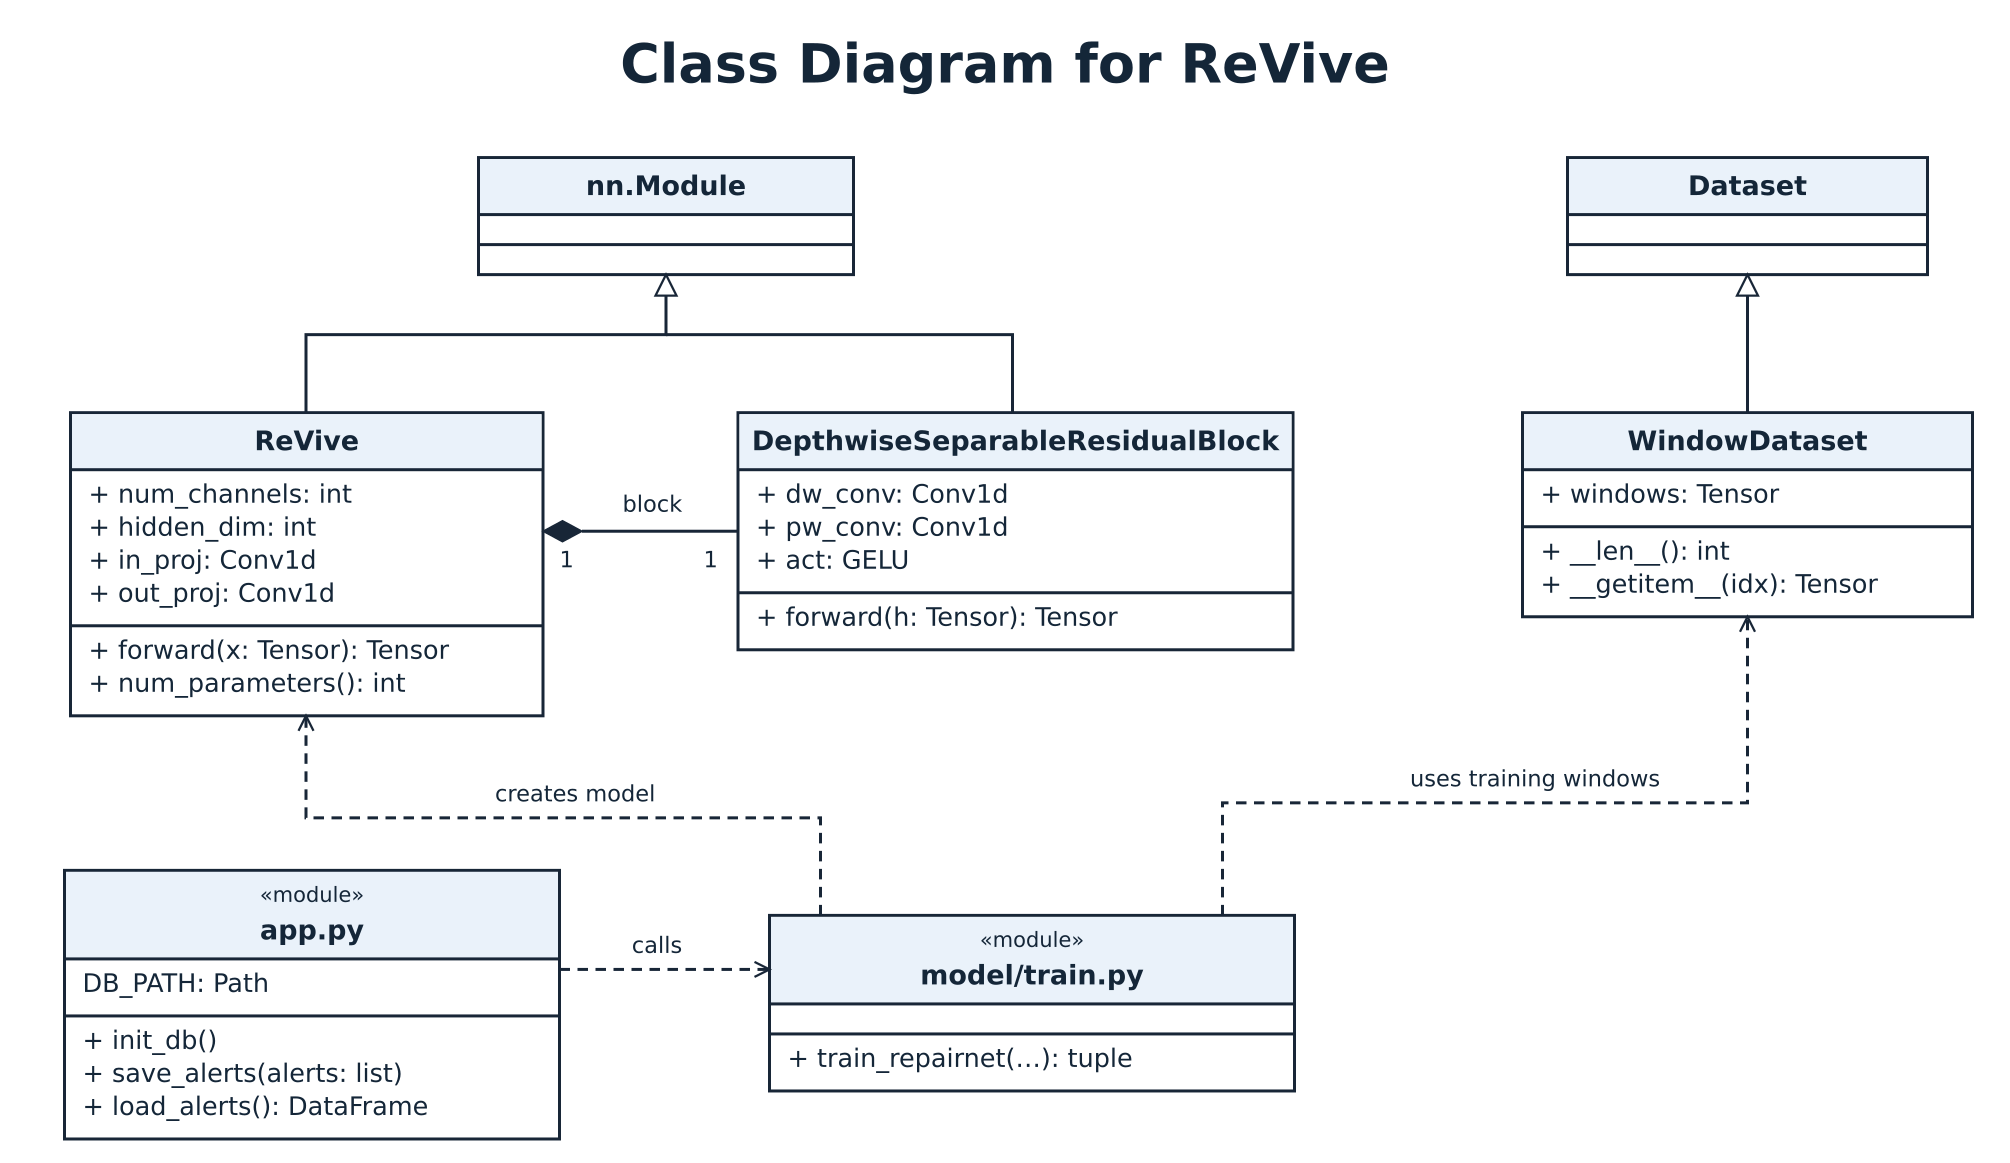
\includegraphics[width=\linewidth,height=0.74\textheight,keepaspectratio]{../docs/images/class-diagram.png}
\end{center}
Model, residual block, and dataset relationships.
\clearpage
\section{Level 0 data flow diagram}
\begin{center}
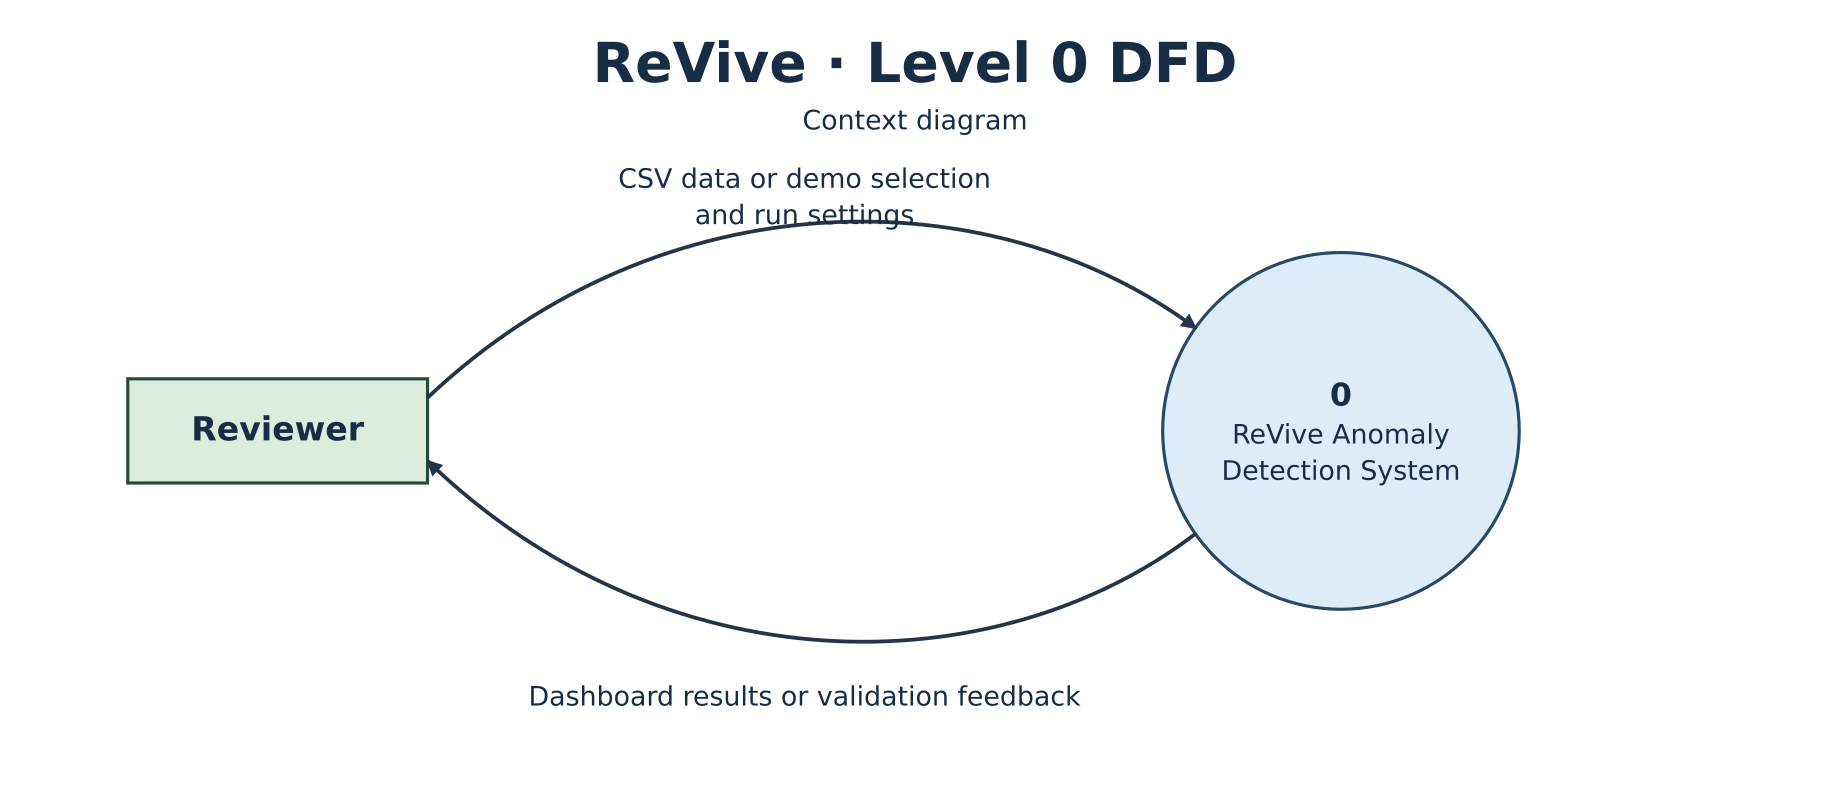
\includegraphics[width=\linewidth,height=0.74\textheight,keepaspectratio]{../docs/images/dfd-level-0.png}
\end{center}
Data exchanged between the Reviewer and ReVive.
\clearpage
\section{Level 1 data flow diagram}
\begin{center}
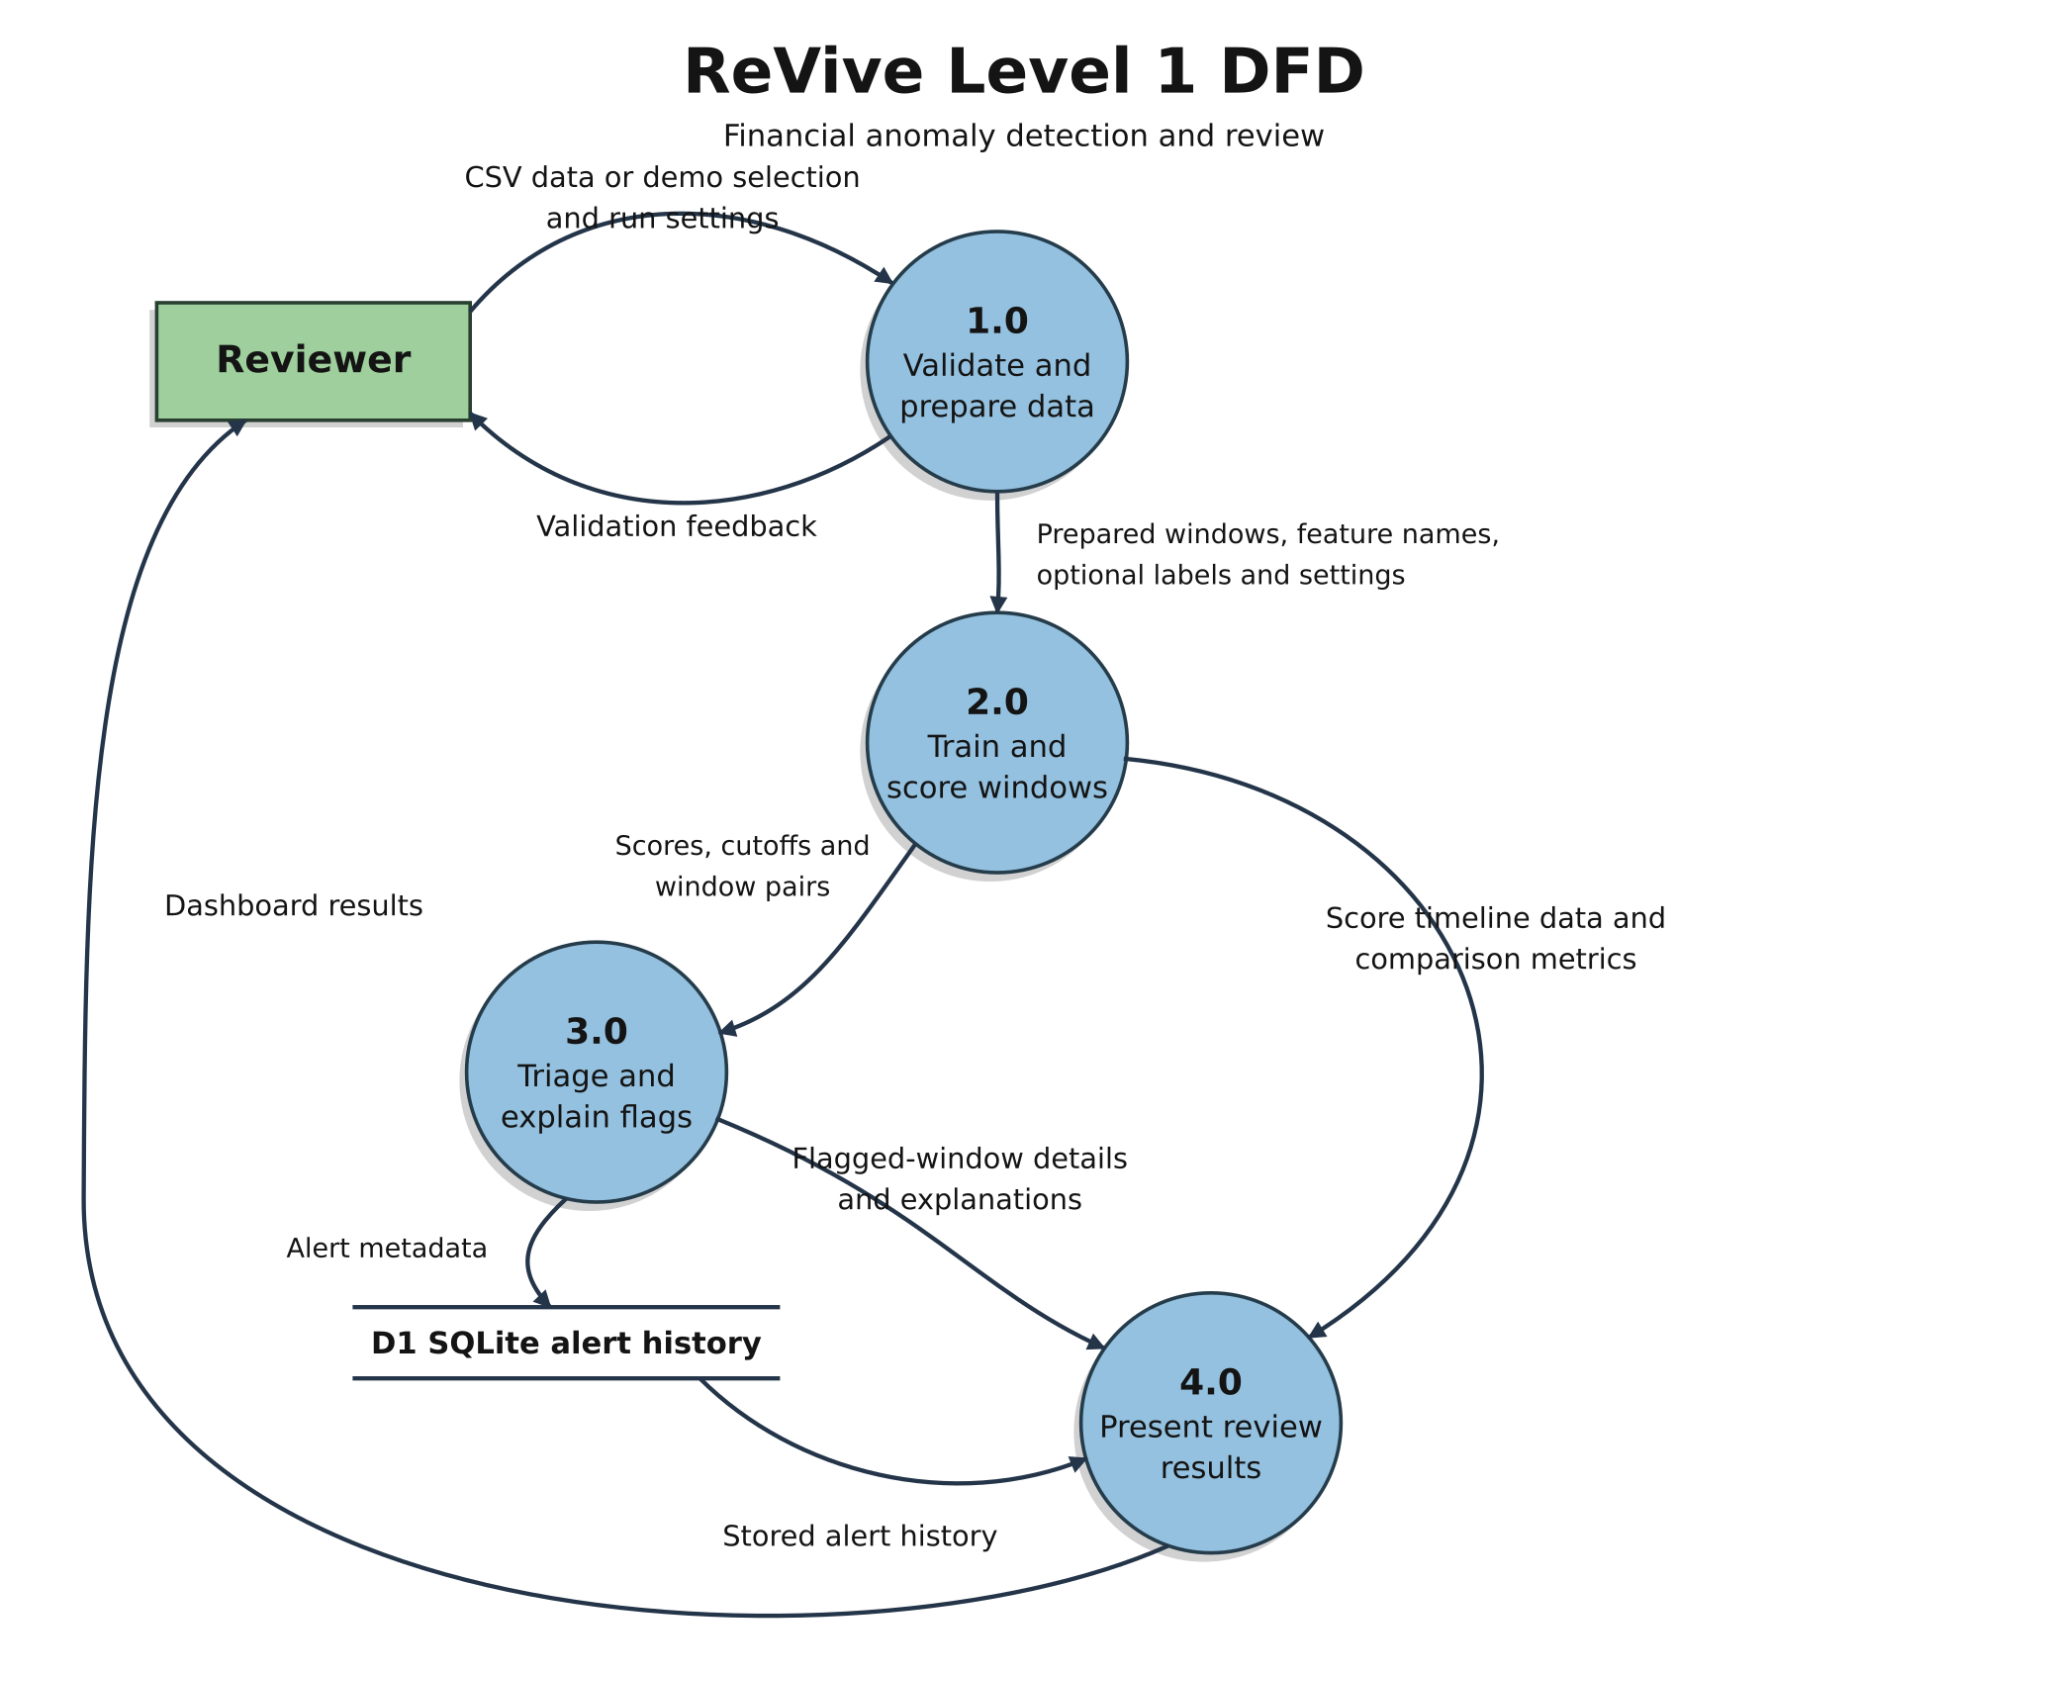
\includegraphics[width=\linewidth,height=0.74\textheight,keepaspectratio]{../docs/images/dfd-level-1.png}
\end{center}
Internal processing, data flows, and alert history.
\clearpage
\section{Sequence diagram}
\begin{center}
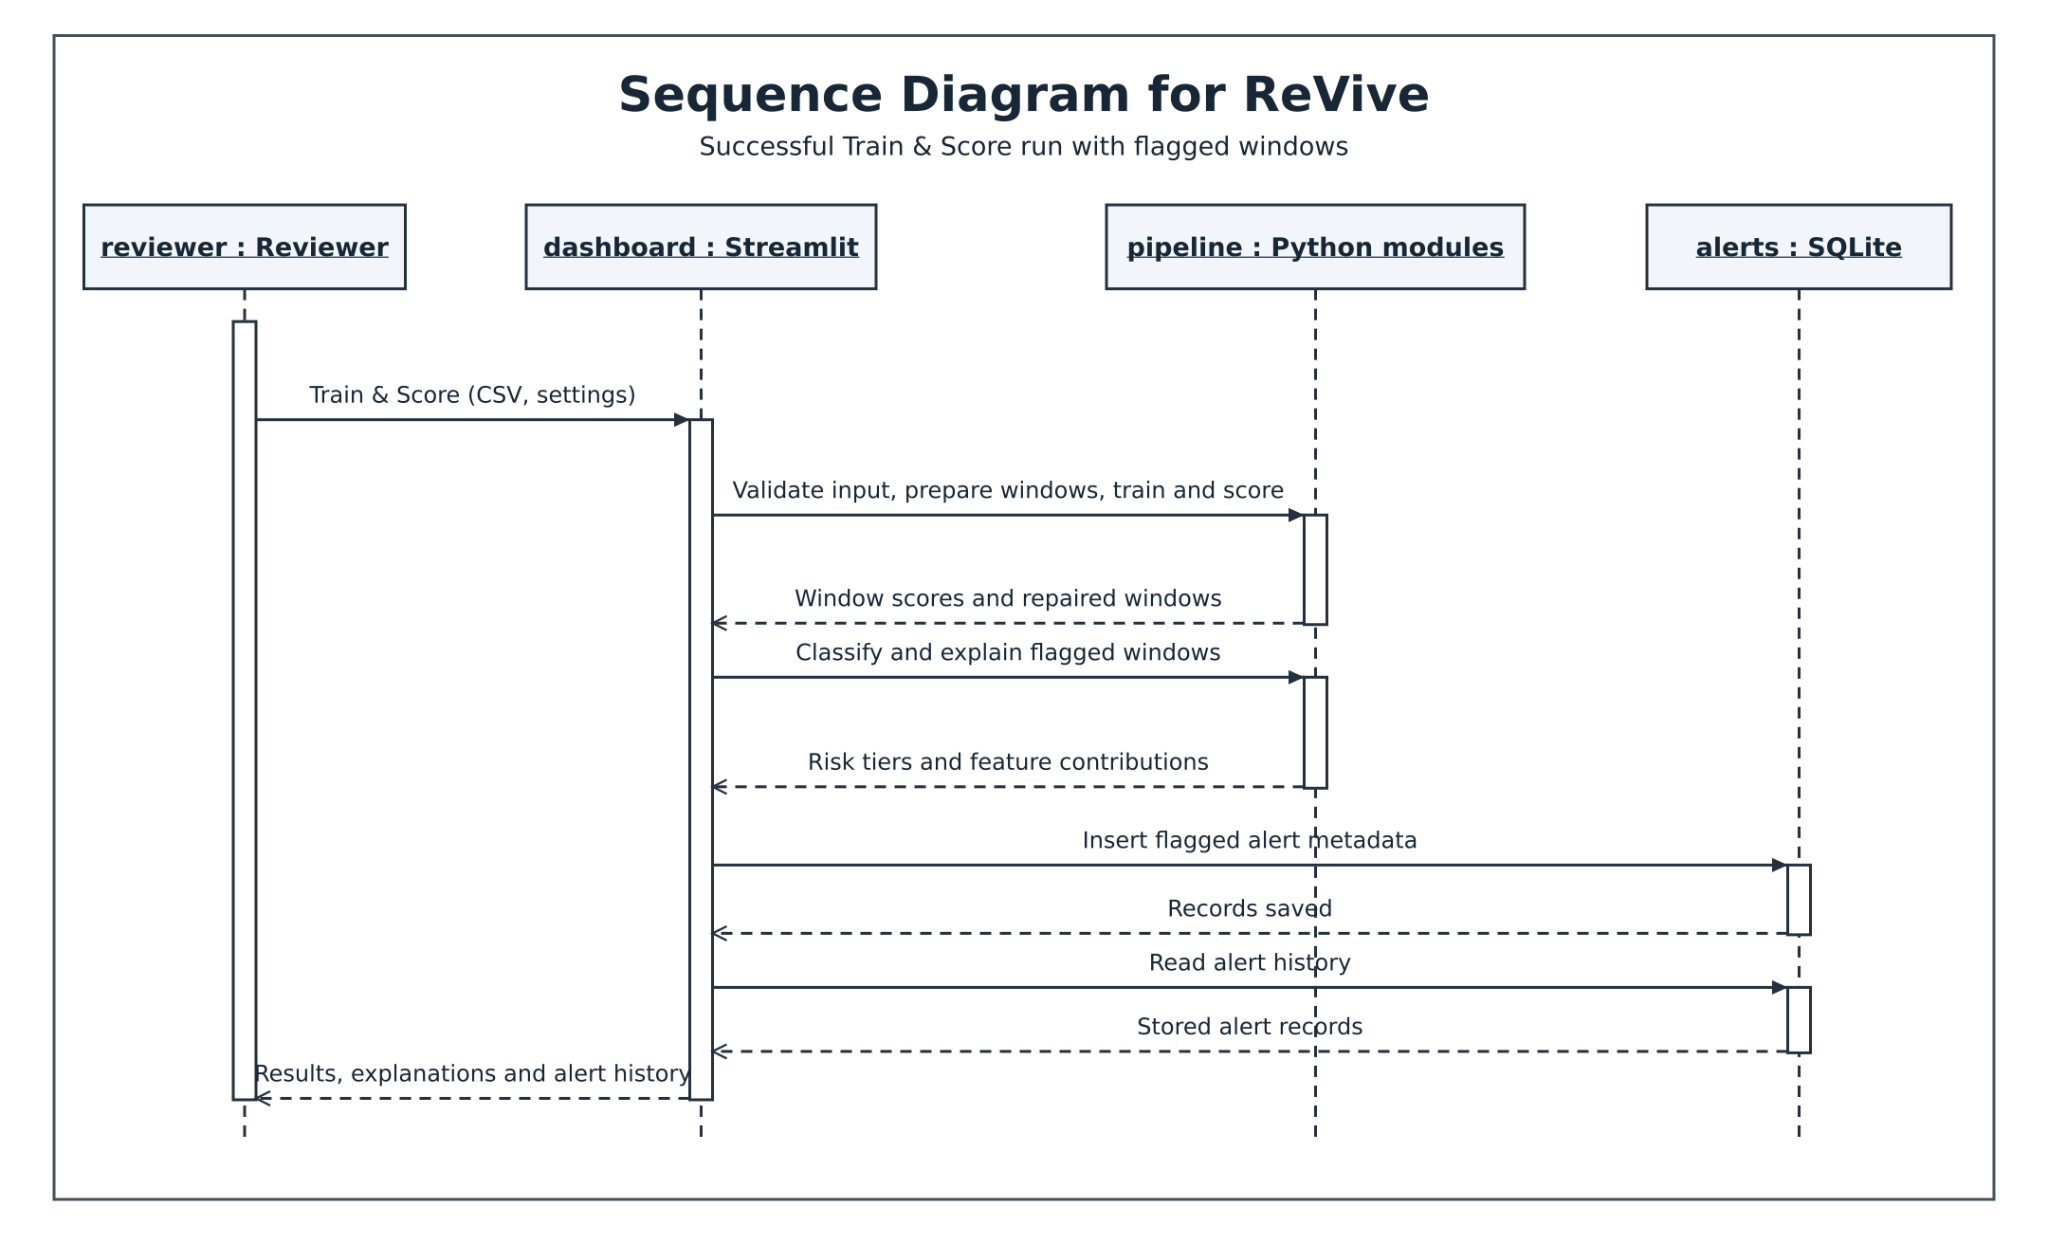
\includegraphics[width=\linewidth,height=0.74\textheight,keepaspectratio]{../docs/images/sequence-diagram.png}
\end{center}
A successful scoring run with flagged windows.
\end{document}
